\documentclass[12pt,a4paper]{article}
\usepackage{tabularx}
\usepackage{ltablex}
\usepackage{graphicx}
\usepackage[cache=false]{minted}
\setminted[erlang]{
frame=lines,
framesep=2mm,
baselinestretch=1.1,
fontsize=\footnotesize,
linenos,
breaklines}
\setminted[haskell]{
frame=lines,
framesep=2mm,
baselinestretch=1.1,
fontsize=\footnotesize,
linenos,
breaklines}
\setminted[bnf]{
frame=lines,
framesep=2mm,
baselinestretch=1.1,
fontsize=\footnotesize,
linenos,
breaklines}
\usemintedstyle{friendly}
% Add Subtitle
\usepackage{titling}
\newcommand{\subtitle}[1]{%
  \posttitle{%
    \par\end{center}
    \begin{center}\large#1\end{center}
    \vskip0.5em}%
}

\begin{document}

\title{Advanced Programming}
\subtitle{Exam 2018}

\author{Silvan Robert Adrian}
\date{\today}
	
\maketitle
\tableofcontents

\section{Question 1.1: Utility functions}
The Code for this task is attached in the appendix \ref{appendix:question1-1}.

\subsection{Version}


\section{Question 1.2: Parsing appm databases}
\subsection{Choice of parser library}
I implemented the Parser for appm in parsec, mostly out of this reason:
\begin{itemize}
	\item Better Error handling compared to ReadP
	\item I do have more experience with Parsec then ReadP
\end{itemize}

\subsection{Transform Grammar}
The existing grammar has some ambiguities, like allowing many names, version etc. which now transformed to only allow once
\begin{minted}{bnf}
Database ::= \epsilon

\end{minted}


\section{Earls of Ravnica}
The code for this task can be found in Appendix
\subsection{Solution}
\subsection{Implementation}
The earls of Ravnica can be seen as a state machine for which I chose to use gen\_statem.
The following states exist:
\begin{itemize}
	\item Under Configuration
	\item Active
	\item Shutting down
\end{itemize}

\begin{figure}[!htb]
	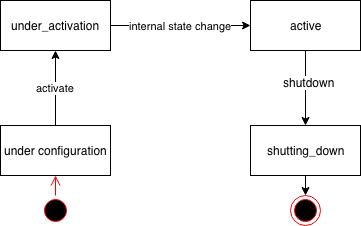
\includegraphics{images/ravnica}
	\caption{Simple State machine diagramm}
\end{figure}

\subsection{Data Structure}
The Data structure I used to implement Ravnica consists of a map with following entries:
\begin{itemize}
	\item \textbf{description} Saves the description which gets saved when starting a server
	\item \textbf{connections} Map for Handling the connections from one District to an other
	\item \textbf{creatures} Map for handling all the entered/active creatures on a Server
\end{itemize}


%\section{Solution}
%\subsection{Files}
%\subsection{Running the programm}
%\subsection{Running the tests}
%\section{Implementation}
%\subsection{Gen-Statem}

%\subsection{Data Structure}
%\subsection{All states}

%\section{Assessment}

%\subsection{Scope of Test Cases}

%\subsection{Correctness}

%\subsection{Code Quality}

\appendix
\section{Code Listing}
\subsection{Question 1.1: handin/appm/src/Utils.hs}
\label{appendix:question1-1}
\inputminted{haskell}{handin/appm/src/Utils.hs}
\subsection{Question 2.1: handin/ravnica/district.erl}
\inputminted{erlang}{handin/ravnica/district.erl}
%\inputminted{erlang}{handin/src/quizmaster_helpers.erl}

\end{document}